%!TEX TS-program = Xelatex  
%!TEX encoding = UTF-8 Unicode  
  
  
\documentclass[12pt]{article}  
\usepackage{geometry}  
\geometry{letterpaper}  
  
\usepackage{fancyhdr} 
\usepackage{layout}
\addtolength{\hoffset}{-1.0cm} \addtolength{\textwidth}{2cm}
\addtolength{\voffset}{-1.0cm} \addtolength{\textheight}{2cm}
\usepackage[rgb]{xcolor}

\usepackage{cite}
\makeatletter
\def\@cite#1#2{\textsuperscript{[{#1\if@tempswa , #2\fi}]}}
\makeatother

\usepackage{listings}
\definecolor{dkgreen}{rgb}{0,0.6,0}
\definecolor{gray}{rgb}{0.5,0.5,0.5}
\definecolor{bcol}{rgb}{0.85,0.85,0.85}
\definecolor{mauve}{rgb}{0.58,0,0.82}
\definecolor{mygray}{gray}{.9}
\definecolor{mypink}{rgb}{.99,.91,.95}
\definecolor{mycyan}{cmyk}{.3,0,0,0}
\usepackage{cite} 
\newcommand{\ucite}[1]
{\textsuperscript{\cite{#1}}}

\lstset{ %
language=python,                % the language of the code
basicstyle=\footnotesize,       % the size of the fonts that are used for the code
numbers=left,                   % where to put the line-numbers
numberstyle=\tiny\color{gray},  % the style that is used for the line-numbers
stepnumber=1,                   % the step between two line-numbers. If it's 1, each line
                                % will be numbered
numbersep=5pt,                  % how far the line-numbers are from the code
backgroundcolor=\color{bcol},   % choose the background color. You must add \usepackage{color}
showspaces=false,               % show spaces adding particular underscores
showstringspaces=false,         % underline spaces within strings
showtabs=false,                 % show tabs within strings adding particular underscores
frame=shadowbox,                % adds a frame around the code
rulecolor=\color{black},        % if not set, the frame-color may be changed on line-breaks within not-black text (e.g. commens (green here))
tabsize=2,                      % sets default tabsize to 2 spaces
captionpos=t,                   % sets the caption-position to bottom
breaklines=true,                % sets automatic line breaking
breakatwhitespace=false,        % sets if automatic breaks should only happen at whitespace
title=\lstname,                     % show the filename of files included with \lstinputlisting;
                                    % also try caption instead of title
keywordstyle=\color{blue},          % keyword style
commentstyle=\color{dkgreen},       % comment style
stringstyle=\color{mauve},          % string literal style
escapeinside=``,                    % if you want to add LaTeX within your code
morekeywords={LONG64,LONGLONG,bool}                % if you want to add more keywords to the set
}



\usepackage{flushend, cuted} %

\usepackage{indentfirst,latexsym,bm}
\usepackage{amsmath,amssymb,amsfonts}
\usepackage{pifont} 
\usepackage{fontspec,xltxtra,xunicode}  
\defaultfontfeatures{Mapping=tex-text}  

\usepackage{algorithmic}
\usepackage[noend, ruled, linesnumbered]{algorithm2e}
\setromanfont{华文宋体} %设置中文字体  
\XeTeXlinebreaklocale “zh”  
\XeTeXlinebreakskip = 0pt plus 1pt minus 0.1pt %文章内中文自动换行  
  
 \setlength{\columnsep}{3em}          %设置分栏间隔
\setlength{\parindent}{2em}          %设置段首缩进量
\renewcommand{\baselinestretch}{1.2} %重设行距     
 \usepackage{graphicx}
\usepackage{cite}
\newcommand{\red}[1]{  \textcolor{red}  {#1}}   %红色\makeatletter
\newcommand{\blue}[1]{ \textcolor{blue} {#1}}   %蓝色\def\@cite#1#2{\textsuperscript{[{#1\if@tempswa , #2\fi}]}}
\newcommand{\green}[1]{\textcolor{green}{#1}}   %绿色\makeatother


% ----------------------------------------------------------------
\vfuzz2pt % Don't report over-full v-boxes if over-edge is small
\hfuzz2pt % Don't report over-full h-boxes if over-edge is small

%%--------------------------------------------------
%% 图片文件路径
%%--------------------------------------------------
\graphicspath{{Figures/}}


% MATH -----------------------------------------------------------
\DeclareMathOperator{\diag}{diag}
\DeclareMathOperator{\rank}{rank}
\DeclareMathOperator{\vecm}{vec}
\DeclareMathOperator{\vecs}{vecs}

\newcommand{\mfloor}[1]{ \left\lfloor {#1} \right\rfloor }
\newcommand{\mpair}[2]{ \left\langle {#1}, {#2} \right\rangle}


\renewcommand{\bf}[1]{\mathbf{#1}}
\renewcommand{\vec}[1]{\bm{#1}}    %向量, 黑斜体
\newcommand{\mat}[1]{\bm{#1}}    %矩阵
\newcommand{\dif}{\mathrm{d}}
\newcommand{\me} {\mathrm{e}}
\newcommand{\mi} {\mathrm{i}}
\newcommand{\vei} {\mathrm{vec}}

\newcommand{\vecmat}[1]{\vecm{\left( #1 \right)}}
\newcommand{\vecsmat}[1]{\vecs{\left( #1 \right)}}
\newcommand{\vecasym}[1]{[#1]_\times}   % antisymmetric matrix from a vector
\newcommand{\id} {\mathbbm{1}}   % identity operator
\newcommand{\fracode}[2]{\frac{\dif {#1}}{\dif {#2}}}         % ordinary differential operator
\newcommand{\fracpde}[2]{\frac{\partial {#1}}{\partial {#2}}} % partial differential operator
\newcommand{\fracpderow}[2]{\partial {#1}/\partial {#2}}
\newcommand{\fracoderow}[2]{\dif {#1}/\dif {#2}}
\newcommand{\fracpdemix}[3]{\frac{\partial^2 {#1}}{\partial {#2} \partial {#3}}}
\newcommand{\lap}[2]{\frac{\partial^2 {#1}}{\partial {#2}^2}}
\newcommand{\laprow}[2]{\partial^2 {#1}/\partial {#2}^2}
\newcommand{\secode}[2]{\frac{\dif^2 {#1}}{\dif {#2}^2}}
\newcommand{\set}[1]{\left\{ #1 \right\}}
\newcommand{\abs}[1]{\left| #1 \right|}
\newcommand{\absvec}[1]{\left| \bf{#1} \right|}
\newcommand{\ket}[1]{|#1 \rangle}
\newcommand{\bra}[1]{\langle #1 |}
\newcommand{\braket}[2]{ \langle #1 | #2 \rangle}
\newcommand{\norm}[1]{\lVert #1 \rVert}
\newcommand{\normF}[1]{{\parallel #1 \parallel}_\textrm{F}}
\newcommand{\trsp}[1]{{#1}^\textsf{T}}
\newcommand{\inv}[1]{#1^{-1}}
\newcommand{\ginv}[1]{#1^+}    % Moore-Penrose (general) inverse
\newcommand{\tinv}[1]{{#1}^{-\textsf{T}}}


\newcommand{\ES}[3]{\mathbb{#1}^{{#2}\times {#3}}}               % Euclidean space
\newcommand{\PS}[3]{\mathbb{#1}^{{#2}\times{#3}}}      % projective space
% ----------------------------------------------------------------
\newfontfamily{\H}{微软雅黑}  
\newfontfamily{\E}{Arial}  


\newfontfamily{\TNR}{Times New Roman}  %设定新的字体快捷命令  
\title{{\H Weekly Report of Research Work\\ }\quad {WR-ABS-TEMP-2015A-No.009}}
\author{汤吉(Ji TANG)\\
               Number: WR-ABS-TEMP-2015A,  E-mail: tangji08@hotmail.com \\
        Date: 18/1/2016 - 24/1/2016}
        \date{January 24, 2016}

  
 %%*************************************************
%%  打印 标题, 作者, 日期等内容
%%*************************************************
\begin{document}  
\maketitle
%%*********************************************
%% 设置页眉与页脚
%%*********************************************
\pagestyle{fancy}
\fancyhead[LO,RE]{\leftmark} % clear all fields
\fancyhead[RO,LE]{WR-ABS-TEMP-2015A-No.009-TJx}   %  请设置正确的个人文档编号



\fancyfoot[LO,RE]{SIAE}
\fancyfoot[RO,RE]{Ji Tang}
\renewcommand{\headrulewidth}{0.4pt}
\renewcommand{\footrulewidth}{0.4pt}



%%*************************************************
%% 显示内容目录
%%*************************************************
\tableofcontents 
\newpage
%%*************************************************
%% 正文部分
%%*************************************************
\section{\H Work}
\begin{enumerate}
	\item Improving all my codes.
	\item Programming the programs to calculate the moving average lines for different periods.
	\item Writing the functions to calculate the Bollinger Bands line and plot it on the Price chart.
	\item Designing a simple GUI calling all the functions I have written.
	\item Choosing a paper and translated a little bit of it.
	\item Learning the Neural Network.
	\item Designing a complete program including setting the parameters, training the data, ploting and GUI for the neural network example.
\end{enumerate}

\section{\H Normalize all my codes}
This week, the first thing I have done is reconstructing all my function in order to have better use of them. 

After this work, the codes are like this:
\begin{lstlisting}
# -*- coding:utf-8 -*-
__author__ = 'Jojo'

import ...
version = sys.version.find("Red Hat")
if version == -1:
    import matplotlib.pyplot as plt

datapath = os.getcwd() + "Data/"

# This function will read the file and translate it to data
# *** the lists of Date, Time, Price ***
def file2data(filename):...


# To calculate the numbers of days between two dates
# *** an int ***
def datediff(beginDate, endDate):...


#This function will set the first data time as the "0" time and format the following data based on this time
# *** a float array ***
def time2number(Date, Time):...


if version == -1:
    # Plot the Data
    # *** No return ***
    def plotforexdata(Date, Time, Price, name):...
    
    
    # Plot the txt by calling the plotforexdata function
    # *** No return ***
    def plotforextxt(filename):...
    
    
# To transform the UTC txt to data
# *** the lists of Time, UTC, Price ***
def UTCfile2data(filename):...


# To transform the UTC txt to data in the giving periode
# *** the lists of Time, UTC, Price ***
def input2data(forextype, startdate, enddate):...


if version == -1:
    # To plot the UTC data with a name
    # *** No return ***
    def plotUTCforexdata(Time, UTC, Price, name):...
    
    
    # To plot the chart in the giving time for the giving type
    # *** No return ***
    def plotpricechart(type, startime, endtime):...
\end{lstlisting}

\section{\H MVA (Moving Average)}
The moving average line is the average value of the giving period line.
\begin{lstlisting}
# code: UTF-8
__author__ = 'Jojo'
from FkNN import *
from changetime import *


# Calculate the moving average line of each period
# *** a matrix of Price and a list of Period ***
def MVA(UTC, Price, Period):
	...
    return MVAPrice, period

if version == -1:
    # Plot the MVA line
    # *** No return ***
    def plotMVAdata(Time, UTC, Price, MVAPrice, period, name):
        ...
        plt.show()


    # To plot the MVA chart in the giving time for the giving type
    # *** No return ***
    def plotMVA(type, startime, endtime, Period):
        ...
        plotMVAdata(Time, UTC, Price, MVAPrice, period, type[-6:])
\end{lstlisting}

\section{\H Bollinger Bands}
\subsection{\H Introduction}
Bollinger Bands is a technical analysis tool invented by John Bollinger in the 1980s as well as a term trademarked by him in 2011.[1] Having evolved from the concept of trading bands, Bollinger Bands and the related indicators %b and bandwidth can be used to measure the "highness" or "lowness" of the price relative to previous trades. Bollinger Bands are a volatility indicator similar to the Keltner channel.

Bollinger Bands consist of:
an N-period moving average (MA)
an upper band at K times an N-period standard deviation above the moving average (MA + Kσ)
a lower band at K times an N-period standard deviation below the moving average (MA − Kσ)

Typical values for N and K are 20 and 2, respectively. The default choice for the average is a simple moving average, but other types of averages can be employed as needed. Exponential moving averages is a common second choice. Usually the same period is used for both the middle band and the calculation of standard deviation.

\subsection{\H Interpretation}
The use of Bollinger Bands varies widely among traders. Some traders buy when price touches the lower Bollinger Band and exit when price touches the moving average in the center of the bands. Other traders buy when price breaks above the upper Bollinger Band or sell when price falls below the lower Bollinger Band. Moreover, the use of Bollinger Bands is not confined to stock traders; options traders, most notably implied volatility traders, often sell options when Bollinger Bands are historically far apart or buy options when the Bollinger Bands are historically close together, in both instances, expecting volatility to revert towards the average historical volatility level for the stock.

When the bands lie close together, a period of low volatility is indicated. Conversely, as the bands expand, an increase in price action/market volatility is indicated. When the bands have only a slight slope and track approximately parallel for an extended time, the price will generally be found to oscillate between the bands as though in a channel.

Traders are often inclined to use Bollinger Bands with other indicators to confirm price action. In particular, the use of oscillator-like Bollinger Bands will often be coupled with a non-oscillator indicator-like chart patterns or a trendline. If these indicators confirm the recommendation of the Bollinger Bands, the trader will have greater conviction that the bands are predicting correct price action in relation to market volatility.\cite{wiki:001}

\subsection{\H Code}
\begin{lstlisting}
# Calculate the moving average line of each period
# *** a matrix of MVA, a 3D-matrix of BOLL and a list of Period ***
def BOLL(UTC, Price, Period):...


# To calculate the moving average value and BOLL values and store it to the "datapath"
# *** No return ***
def saveBOLL(type, startime, endtime, Period):...


    # Plot the BOLL line
    # *** No return ***
    def plotBOLLdata(Time, UTC, Price, MVAPrice, BOLLline, period, name):...
    
    
    # To plot the BOLL chart in the giving time for the giving type
    # *** No return ***
    def plotBOLL(type, startime, endtime, Period):...
\end{lstlisting}

\section{\H GUI for ploting the chart}

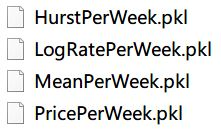
\includegraphics[width=3.5in]{1.jpg}

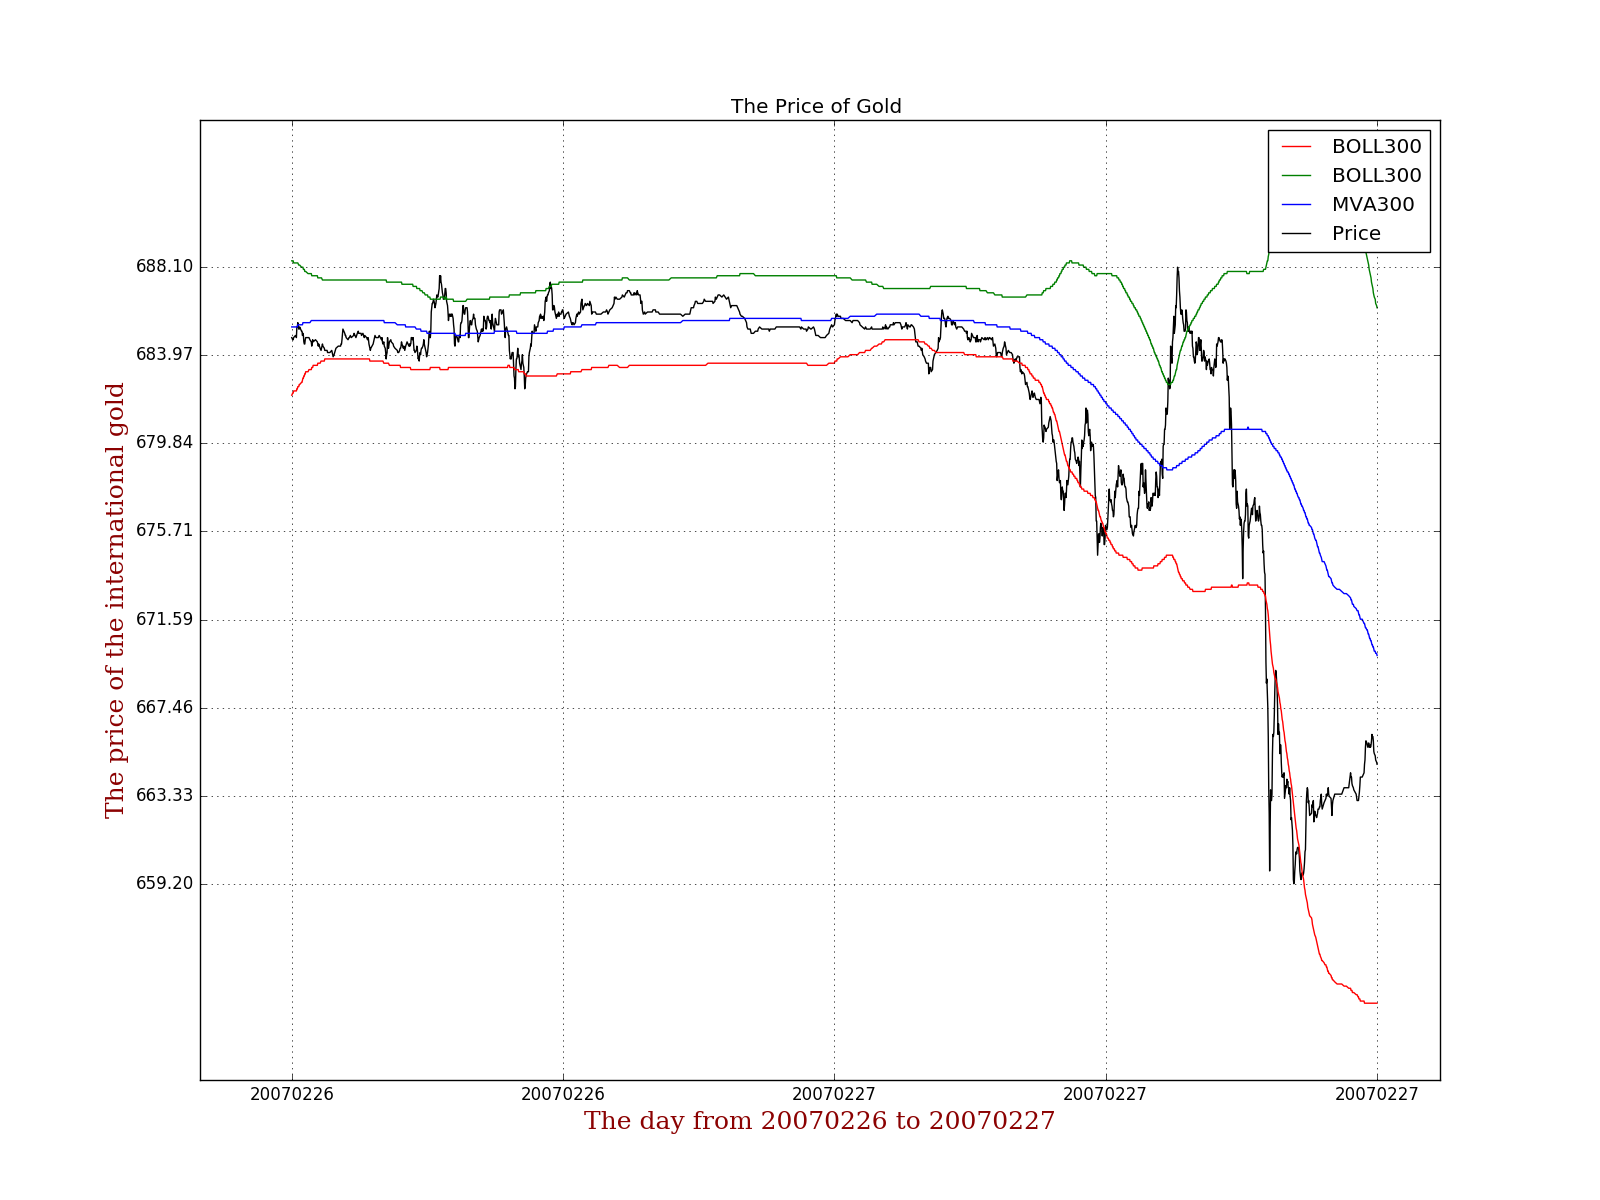
\includegraphics[width=5.5in]{2.png}

\section{\H The paper I select}
I have select a paper named "Hurst exponent and Financial Market Predictability", and begin to translate it.

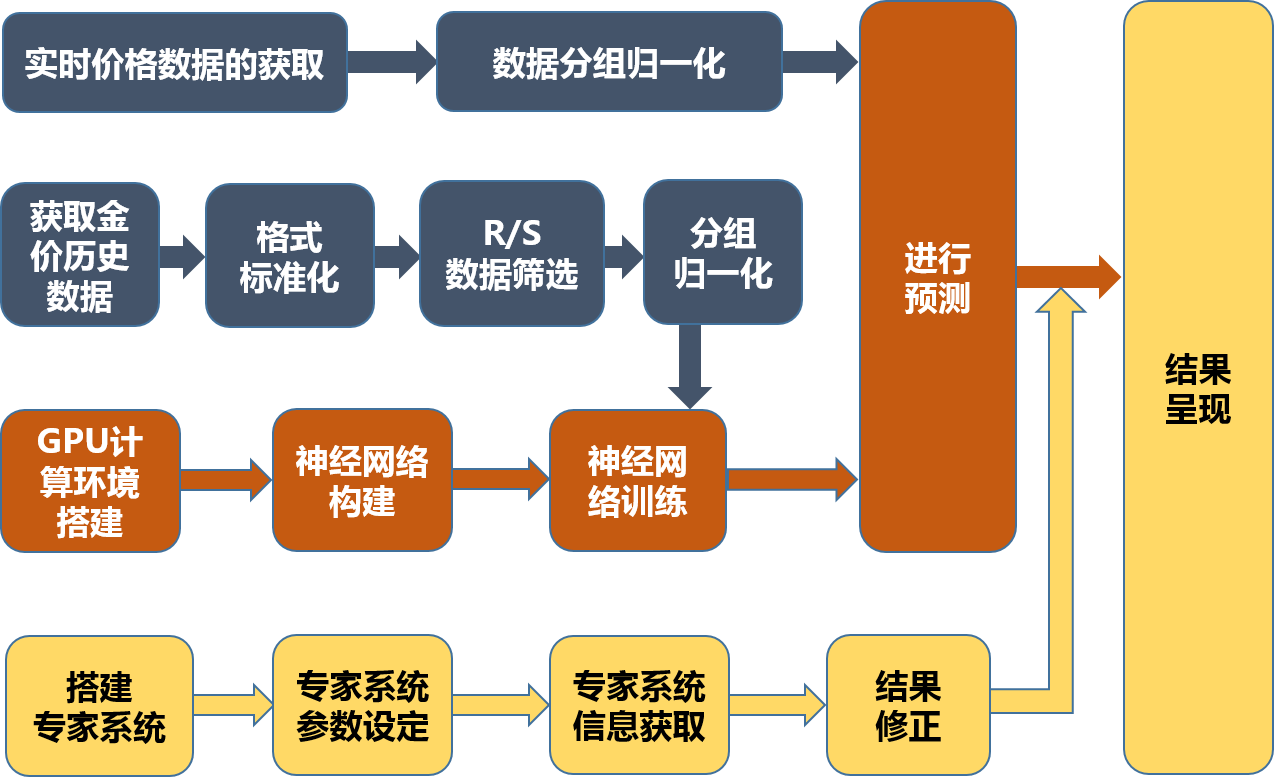
\includegraphics[width=6.5in]{3.jpg}

\section{\H Artificial neural network}
\subsection{\H Background}
Examinations of humans' central nervous systems inspired the concept of artificial neural networks. In an artificial neural network, simple artificial nodes, known as "neurons", "neurodes", "processing elements" or "units", are connected together to form a network which mimics a biological neural network.

There is no single formal definition of what an artificial neural network is. However, a class of statistical models may commonly be called "neural" if it possesses the following characteristics:
1.contains sets of adaptive weights, i.e. numerical parameters that are tuned by a learning algorithm, and
2.capability of approximating non-linear functions of their inputs.

The adaptive weights can be thought of as connection strengths between neurons, which are activated during training and prediction.

Neural networks are similar to biological neural networks in the performing of functions collectively and in parallel by the units, rather than there being a clear delineation of subtasks to which individual units are assigned. The term "neural network" usually refers to models employed in statistics, cognitive psychology and artificial intelligence. Neural network models which command the central nervous system and the rest of the brain are part of theoretical neuroscience and computational neuroscience.\cite{wiki:002}

In modern software implementations of artificial neural networks, the approach inspired by biology has been largely abandoned for a more practical approach based on statistics and signal processing. In some of these systems, neural networks or parts of neural networks (like artificial neurons) form components in larger systems that combine both adaptive and non-adaptive elements. While the more general approach of such systems is more suitable for real-world problem solving, it has little to do with the traditional, artificial intelligence connectionist models. What they do have in common, however, is the principle of non-linear, distributed, parallel and local processing and adaptation. Historically, the use of neural network models marked a directional shift in the late eighties from high-level (symbolic) artificial intelligence, characterized by expert systems with knowledge embodied in if-then rules, to low-level (sub-symbolic) machine learning, characterized by knowledge embodied in the parameters of a dynamical system.

\subsection{\H Improvement}
Computational devices have been created in CMOS, for both biophysical simulation and neuromorphic computing. More recent efforts show promise for creating nanodevices for very large scale principal components analyses and convolution. If successful, these efforts could usher in a new era of neural computing that is a step beyond digital computing, because it depends on learning rather than programming and because it is fundamentally analog rather than digital even though the first instantiations may in fact be with CMOS digital devices.

Between 2009 and 2012, the recurrent neural networks and deep feedforward neural networks developed in the research group of Jürgen Schmidhuber at the Swiss AI Lab IDSIA have won eight international competitions in pattern recognition and machine learning. For example, the bi-directional and multi-dimensional long short term memory (LSTM) of Alex Graves et al. won three competitions in connected handwriting recognition at the 2009 International Conference on Document Analysis and Recognition (ICDAR), without any prior knowledge about the three different languages to be learned.

Fast GPU-based implementations of this approach by Dan Ciresan and colleagues at IDSIA have won several pattern recognition contests, including the IJCNN 2011 Traffic Sign Recognition Competition, the ISBI 2012 Segmentation of Neuronal Structures in Electron Microscopy Stacks challenge, and others. Their neural networks also were the first artificial pattern recognizers to achieve human-competitive or even superhuman performance on important benchmarks such as traffic sign recognition (IJCNN 2012), or the MNIST handwritten digits problem of Yann LeCun at NYU.

Deep, highly nonlinear neural architectures similar to the 1980 neocognitron by Kunihiko Fukushima and the "standard architecture of vision", inspired by the simple and complex cells identified by David H. Hubel and Torsten Wiesel in the primary visual cortex, can also be pre-trained by unsupervised methods of Geoff Hinton's lab at University of Toronto. A team from this lab won a 2012 contest sponsored by Merck to design software to help find molecules that might lead to new drugs.\cite{wiki:003}

\subsection{\H Full Code}
I have selected a python tool named "pybrain" to realize the artificial neural network.
\begin{lstlisting}
#!/usr/bin/env python
#coding:utf-8
from pybrain.datasets import ClassificationDataSet
from pybrain.utilities import percentError
from pybrain.datasets import SupervisedDataSet
from pybrain.tools.shortcuts import buildNetwork
from pybrain.supervised.trainers import BackpropTrainer
from pybrain.structure.modules import SoftmaxLayer
from numpy import *
import matplotlib.pyplot as plt
from mpl_toolkits.mplot3d import Axes3D
import numpy as np
import os
from Tkinter import *
import matplotlib
from matplotlib.backends.backend_tkagg import FigureCanvasTkAgg
from matplotlib.figure import Figure

datapath = os.getcwd()[0:-6] + "/kNN/"
#----------------------------------------------------------------------
def file2matrix(filename):
   fr = open(filename) #Load the data
   NumbersOfLines = len(fr.readlines()) #Get the number of the lines
   returnMatrix = zeros((NumbersOfLines, 3)) #Create Numpy matrix to return
   classLabelVector = []
   fr = open(filename) #Reload the data
   index = 0
   for line in fr.readlines():
      lines = line.strip() #Strip the beginning and the end blank
      listFromLine = lines.split() #Separate each line by '\t'
      returnMatrix[index, :] = listFromLine[0:3] #Get the 3 values of each line
      classLabelVector.append(float(listFromLine[-1])) #Get the evaluate of each person
      index += 1
   return returnMatrix, classLabelVector
def autoNorm(dataSet):
   minValues = dataSet.min(0) #The min value
   maxValues = dataSet.max(0) #The max value
   ranges = maxValues - minValues
   # normDataset = zeros(shape(dataSet))
   m = dataSet.shape[0] #The number of lines
   normDataset = dataSet - tile(minValues, (m, 1))
   normDataset = normDataset/tile(ranges, (m, 1)) #Calculate the values normalized
   return normDataset, ranges, minValues

def drawPic():
    try:
        sampleCount = int(inputEntry.get())
    except:
        sampleCount = 50
        print 'Enter an integer.'
        inputEntry.delete(0, END)
        inputEntry.insert(0, '50')
    # Need column vectors in dataset, not arrays
    for i in range(sampleCount):
        trainer.trainEpochs(1)
        trnresult = percentError(trainer.testOnClassData(), trndata['class'])
        tstresult = percentError(trainer.testOnClassData(dataset=tstdata), tstdata['class'])
        if i % 20 == 0:
            t.delete(1.0, END)
        t.insert(END, "epoch:" + str(trainer.totalepochs) + "  train error:" + str(round(trnresult, 2)) \
                  + "%  test error:" + str(round(tstresult, 2)) + "%\n")
        # Clear the Figure
        drawPic.f.clf()
        drawPic.a = drawPic.f.add_subplot(111, projection='3d')
        drawPic.a.set_title('Training...')
        for a, c, m in [(0, 'r', 'o'), (1, 'b', '^'), (2, 'y', 's')]:
            out = fnn.activateOnDataset(alldata)
            out = out.argmax(axis=1)
            here = (out == a)
            drawPic.a.scatter(alldata['input'][here, 0], alldata['input'][here, 1], alldata['input'][here, 2], c=c, marker=m)
        drawPic.canvas.show()

if __name__ == '__main__':
    matplotlib.use('TkAgg')
    root = Tk()
    root.title('Neural network training')
    new = Tk()
    new.title('Note the errors')
    new.geometry('350x800')
    t = Text(new)
    t.grid(row=1, column=1, rowspan=50, columnspan=50)
    t.pack()
    # Putting a figure on GUI
    drawPic.f = Figure(figsize=(10, 7), dpi=108, facecolor="white")
    ax = drawPic.f.add_subplot(111, projection='3d')
    drawPic.canvas = FigureCanvasTkAgg(drawPic.f, master=root)
    drawPic.canvas.show()
    drawPic.canvas.get_tk_widget().grid(row=0, columnspan=3)
    # Setting Labels and Text
    Label(root, text='Training times:').grid(row=1, column=0)
    inputEntry = Entry(root)
    inputEntry.grid(row=1, column=1)
    inputEntry.insert(0, '50')
    Button(root, text='Begin', command=drawPic).grid(row=1, column=2, columnspan=3)

    alldata = ClassificationDataSet(3, 1, nb_classes=3)
    datingDataMat, datingLabels = file2matrix(datapath + 'datingTestSet.txt')
    normMat, ranges, minValues = autoNorm(datingDataMat)
    for i in range(len(normMat)):
        alldata.addSample(normMat[i], [datingLabels[i] - 1])
    tstdata, trndata = alldata.splitWithProportion(0.25)
    trndata._convertToOneOfMany( )
    tstdata._convertToOneOfMany( )
    alldata._convertToOneOfMany( )
    t.insert(END, "Number of training patterns: " + str(len(trndata)) + "\n")
    t.insert(END, "Input and output dimensions: " + str(trndata.indim) + str(trndata.outdim) + "\n")
    fnn = buildNetwork(trndata.indim, 100, 5, trndata.outdim, outclass=SoftmaxLayer)
    fnn.activate([3, 100, 1])
    trainer = BackpropTrainer(fnn, dataset=trndata, momentum=0.01, verbose=True, weightdecay=0.0001)
    # Begin the loop
    root.mainloop()
\end{lstlisting}

\subsection{\H Test}
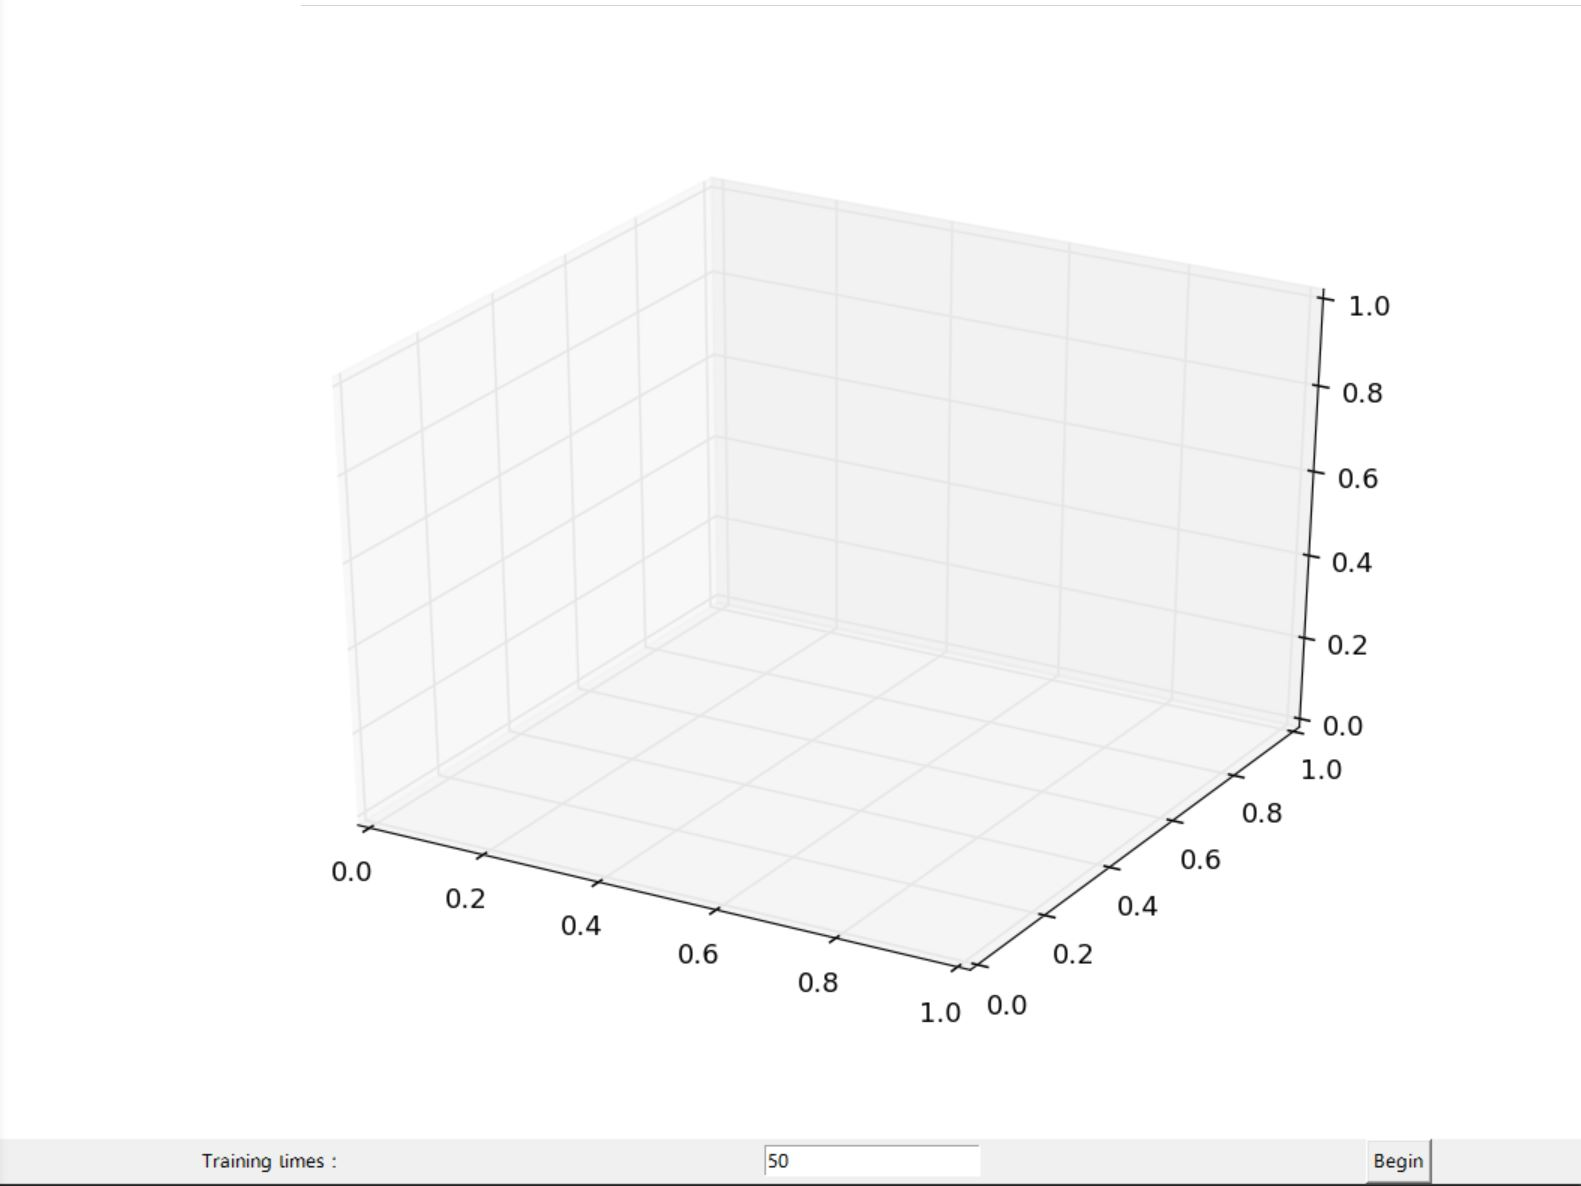
\includegraphics[width=3.5in]{01.jpg}
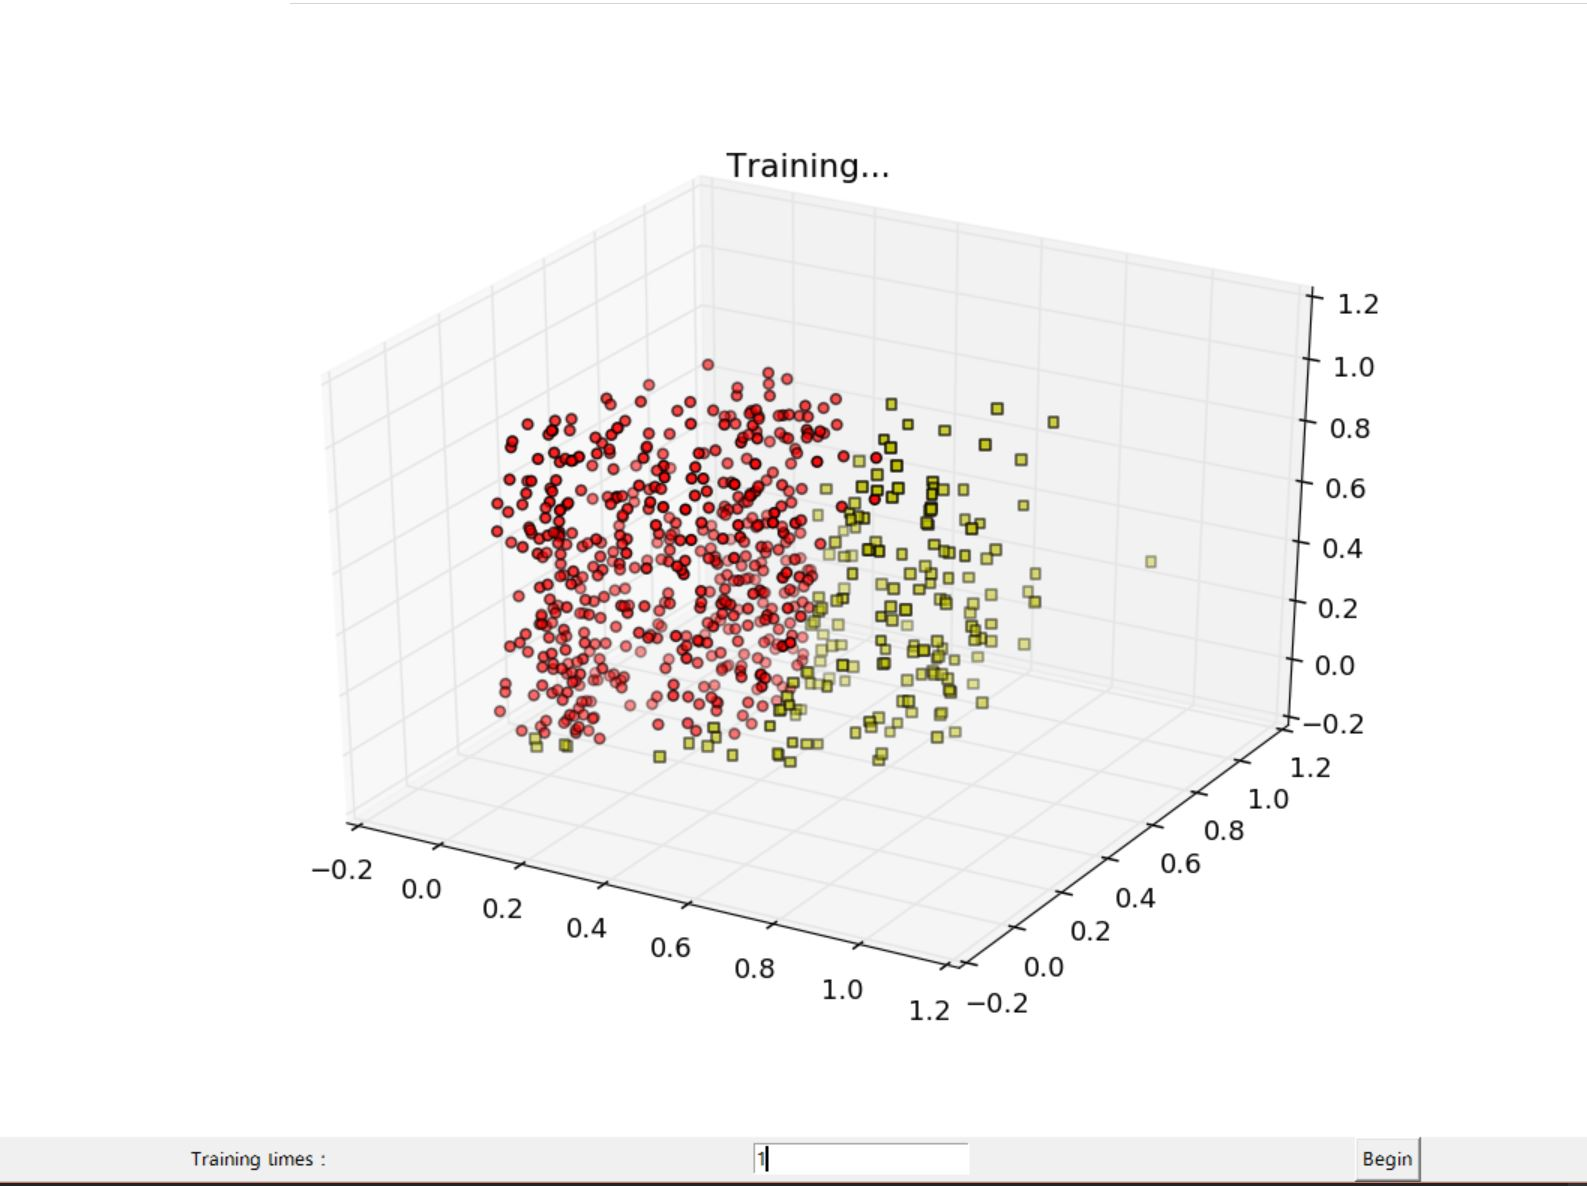
\includegraphics[width=3.5in]{02.jpg}

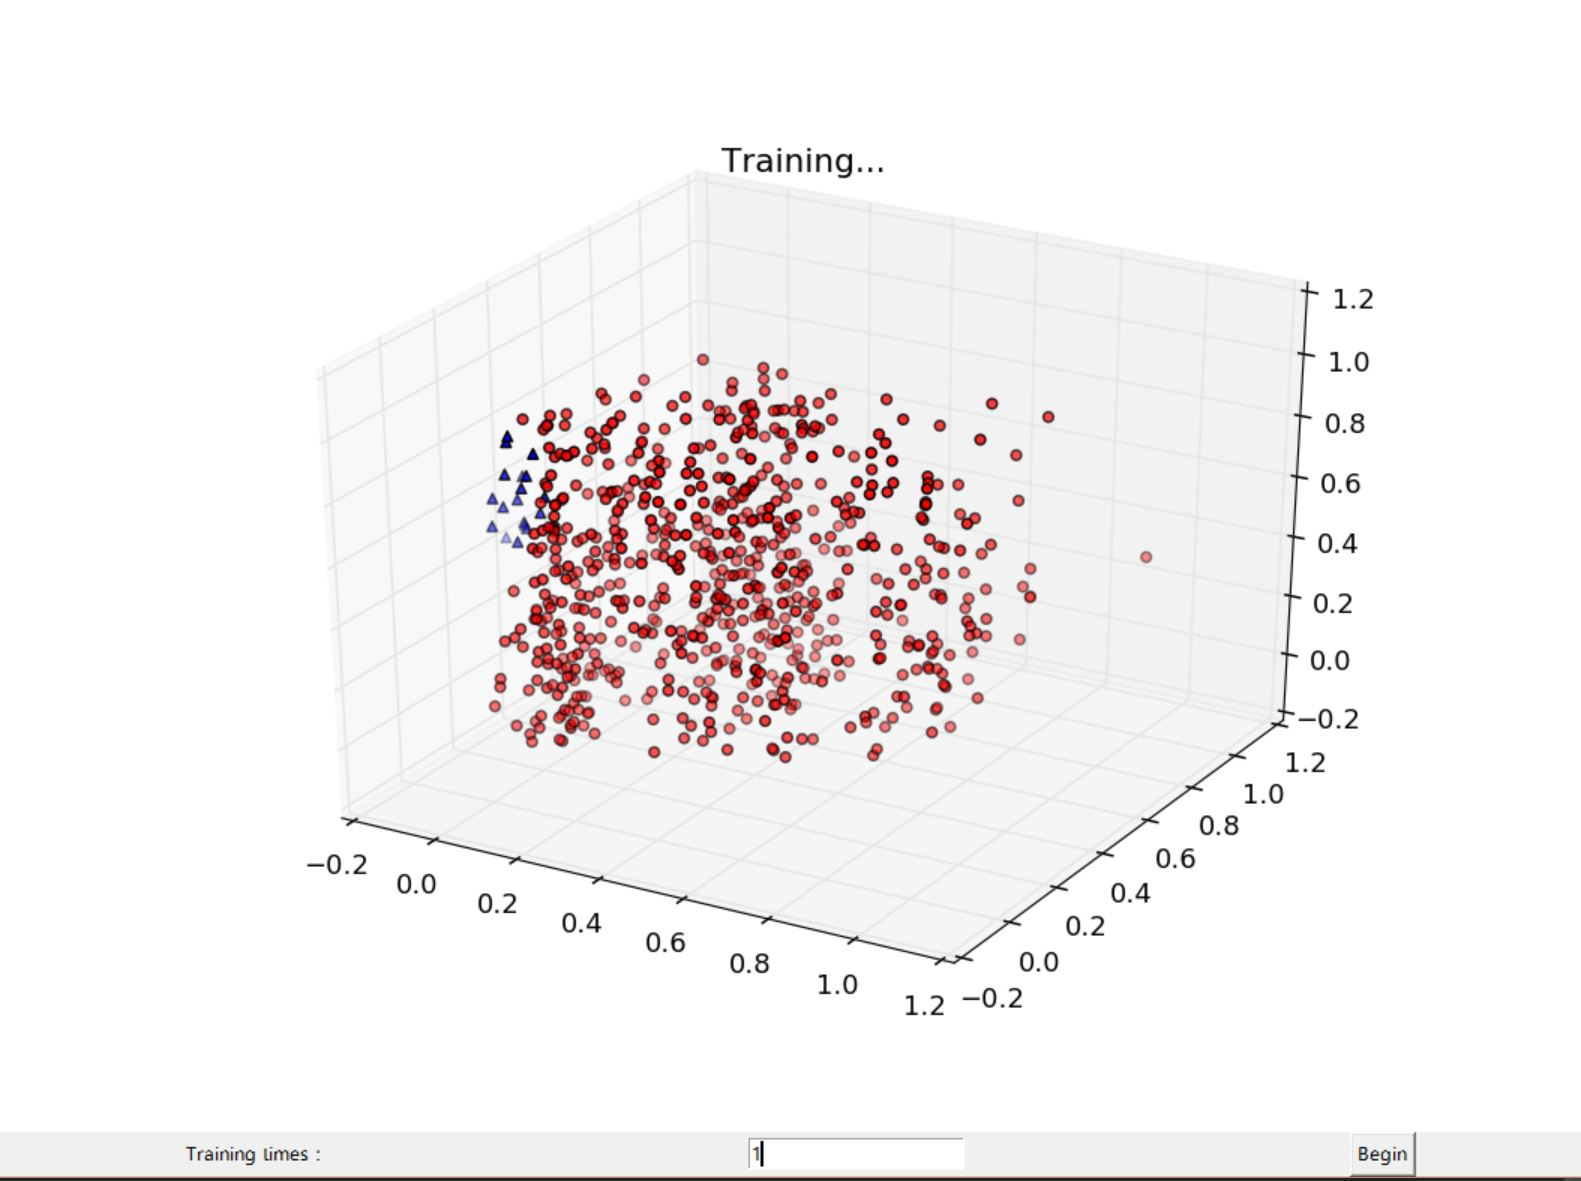
\includegraphics[width=3.5in]{03.jpg}
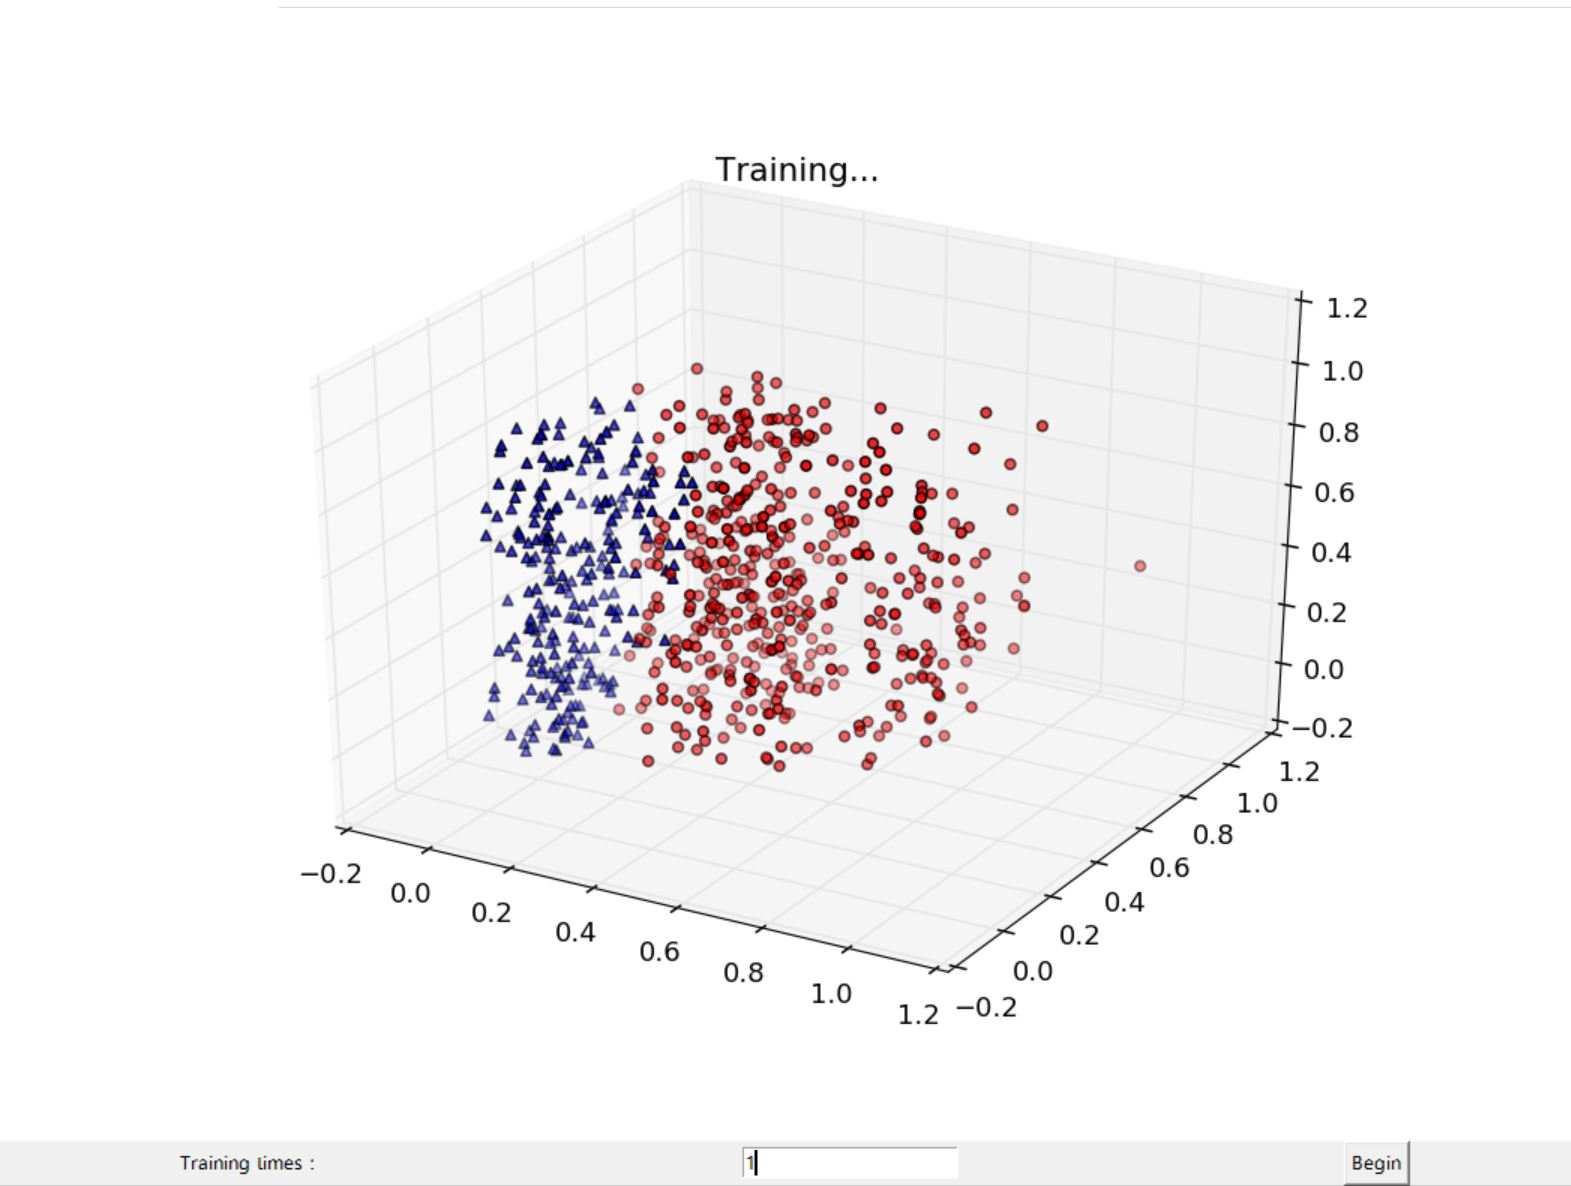
\includegraphics[width=3.5in]{04.jpg}

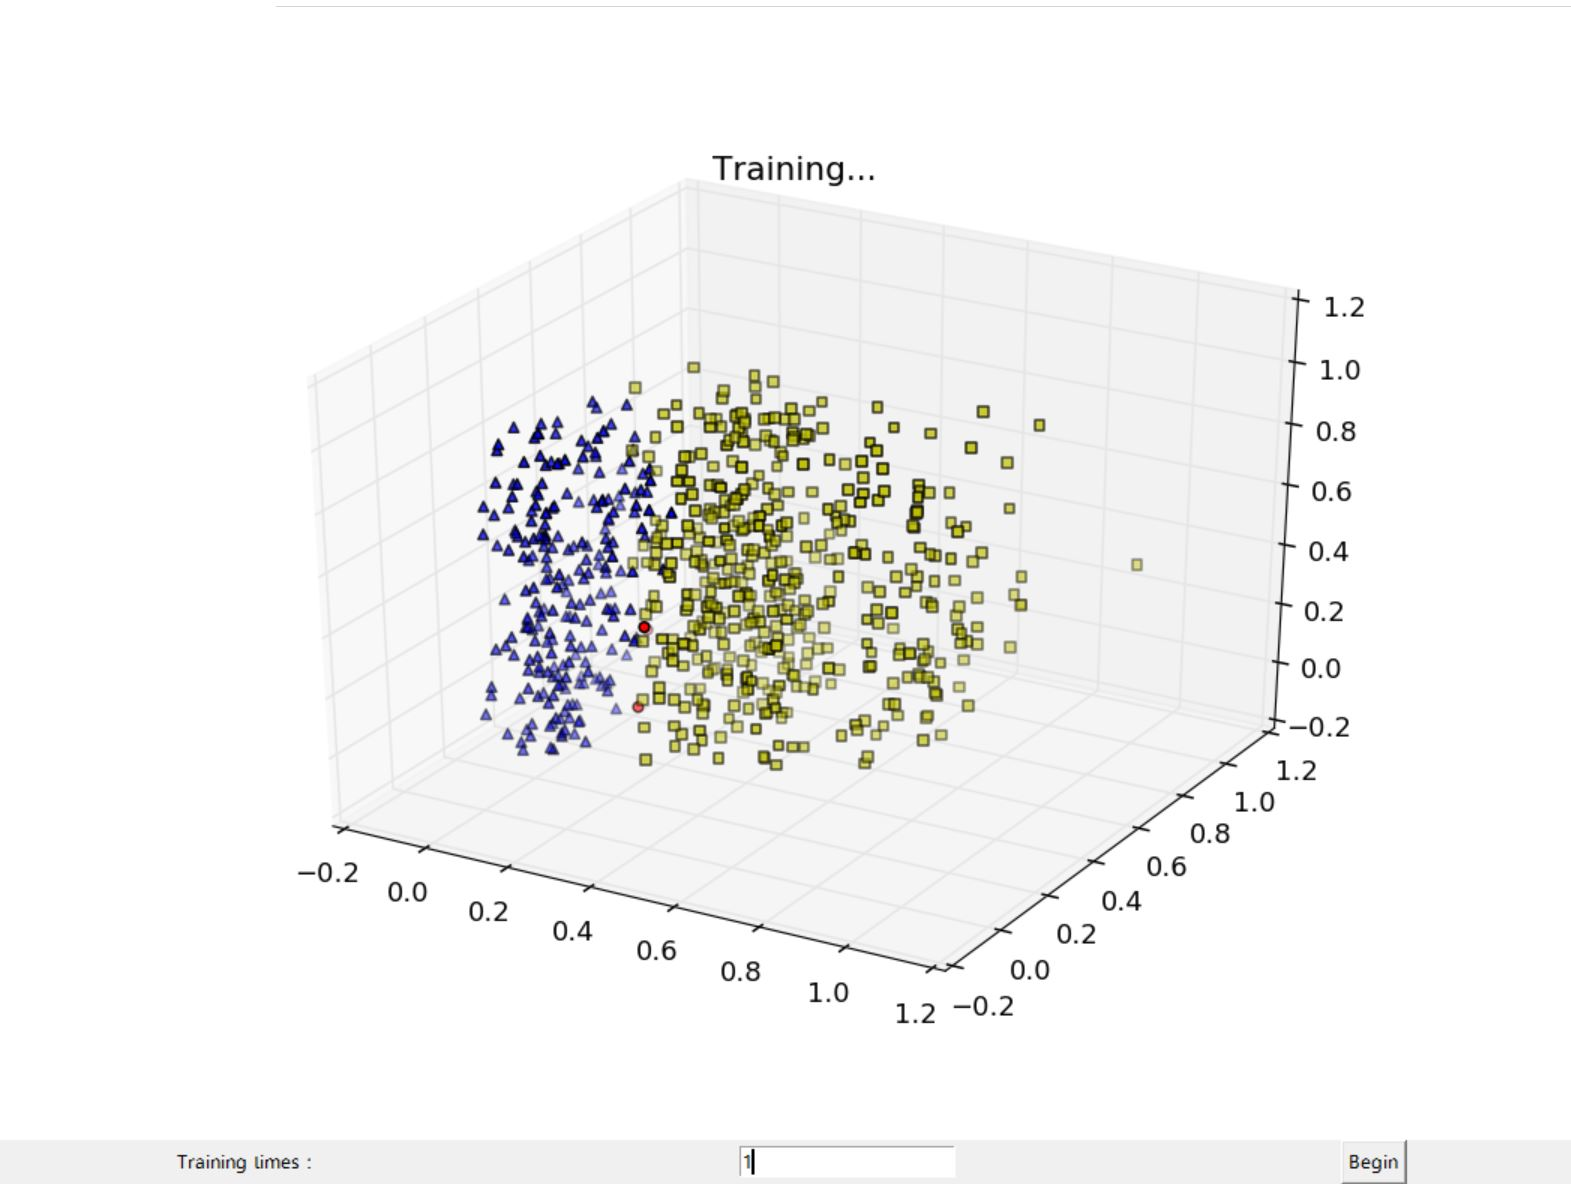
\includegraphics[width=3.5in]{05.jpg}
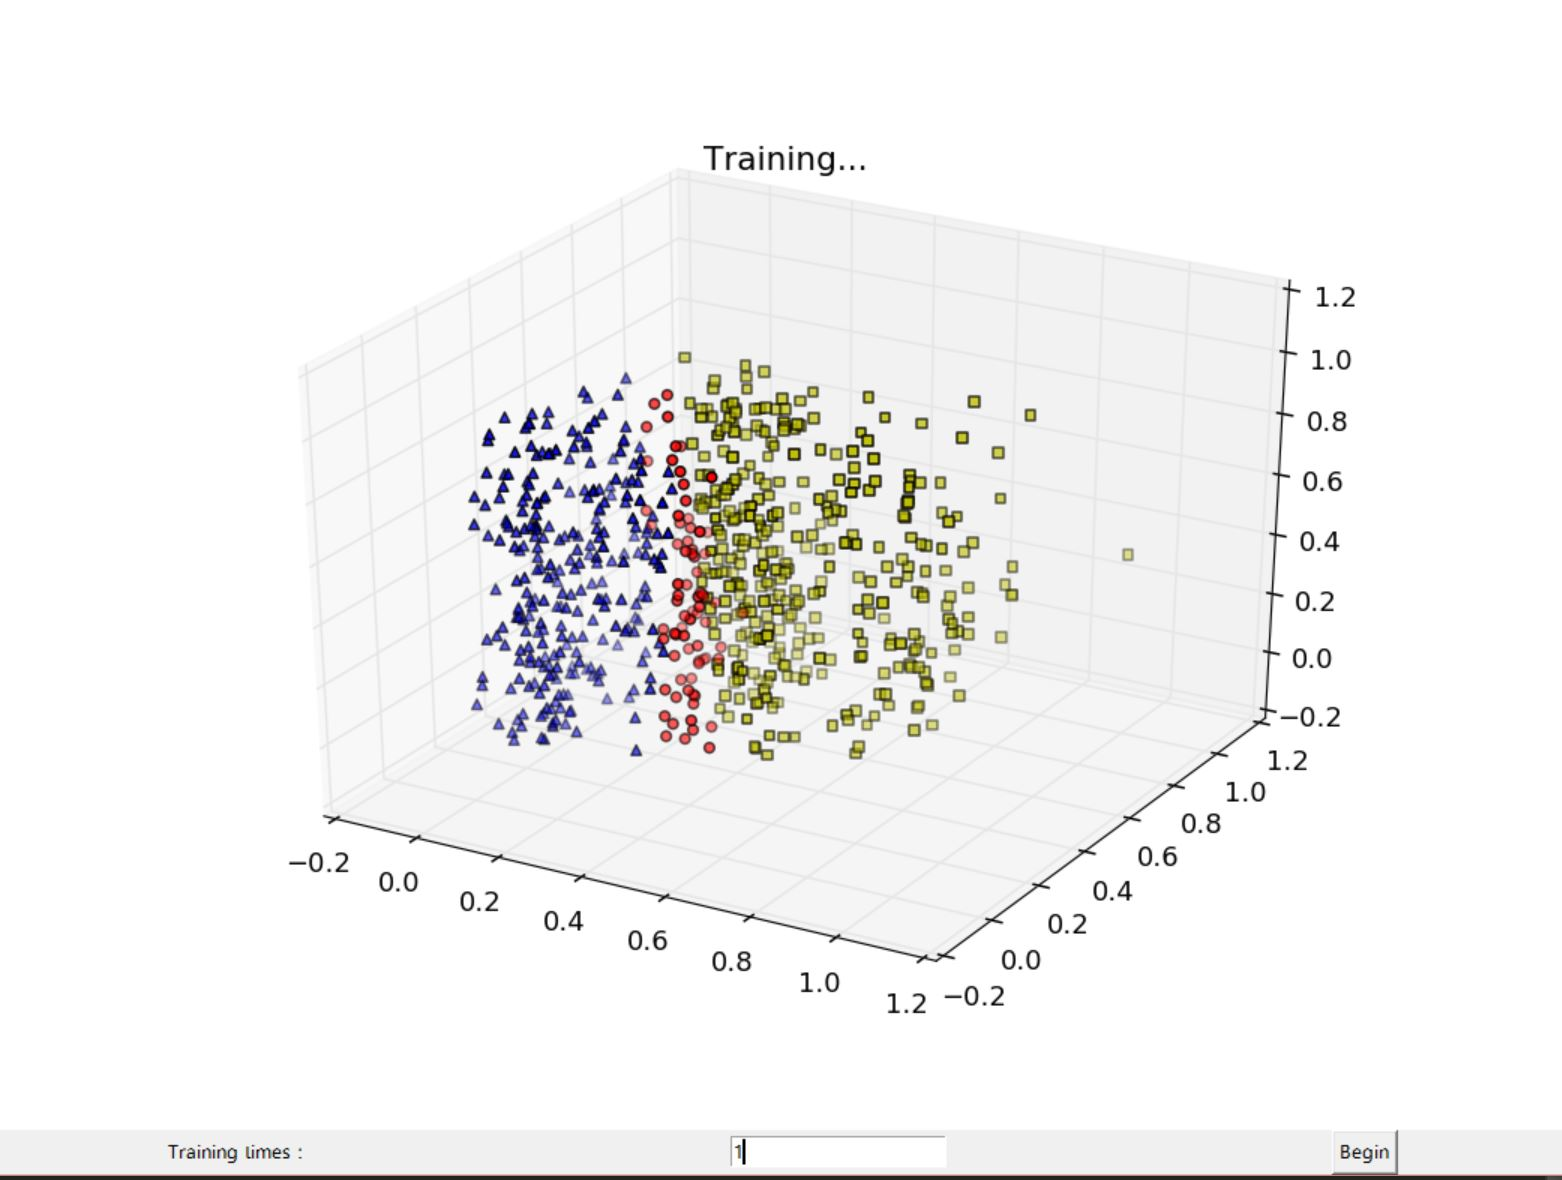
\includegraphics[width=3.5in]{06.jpg}

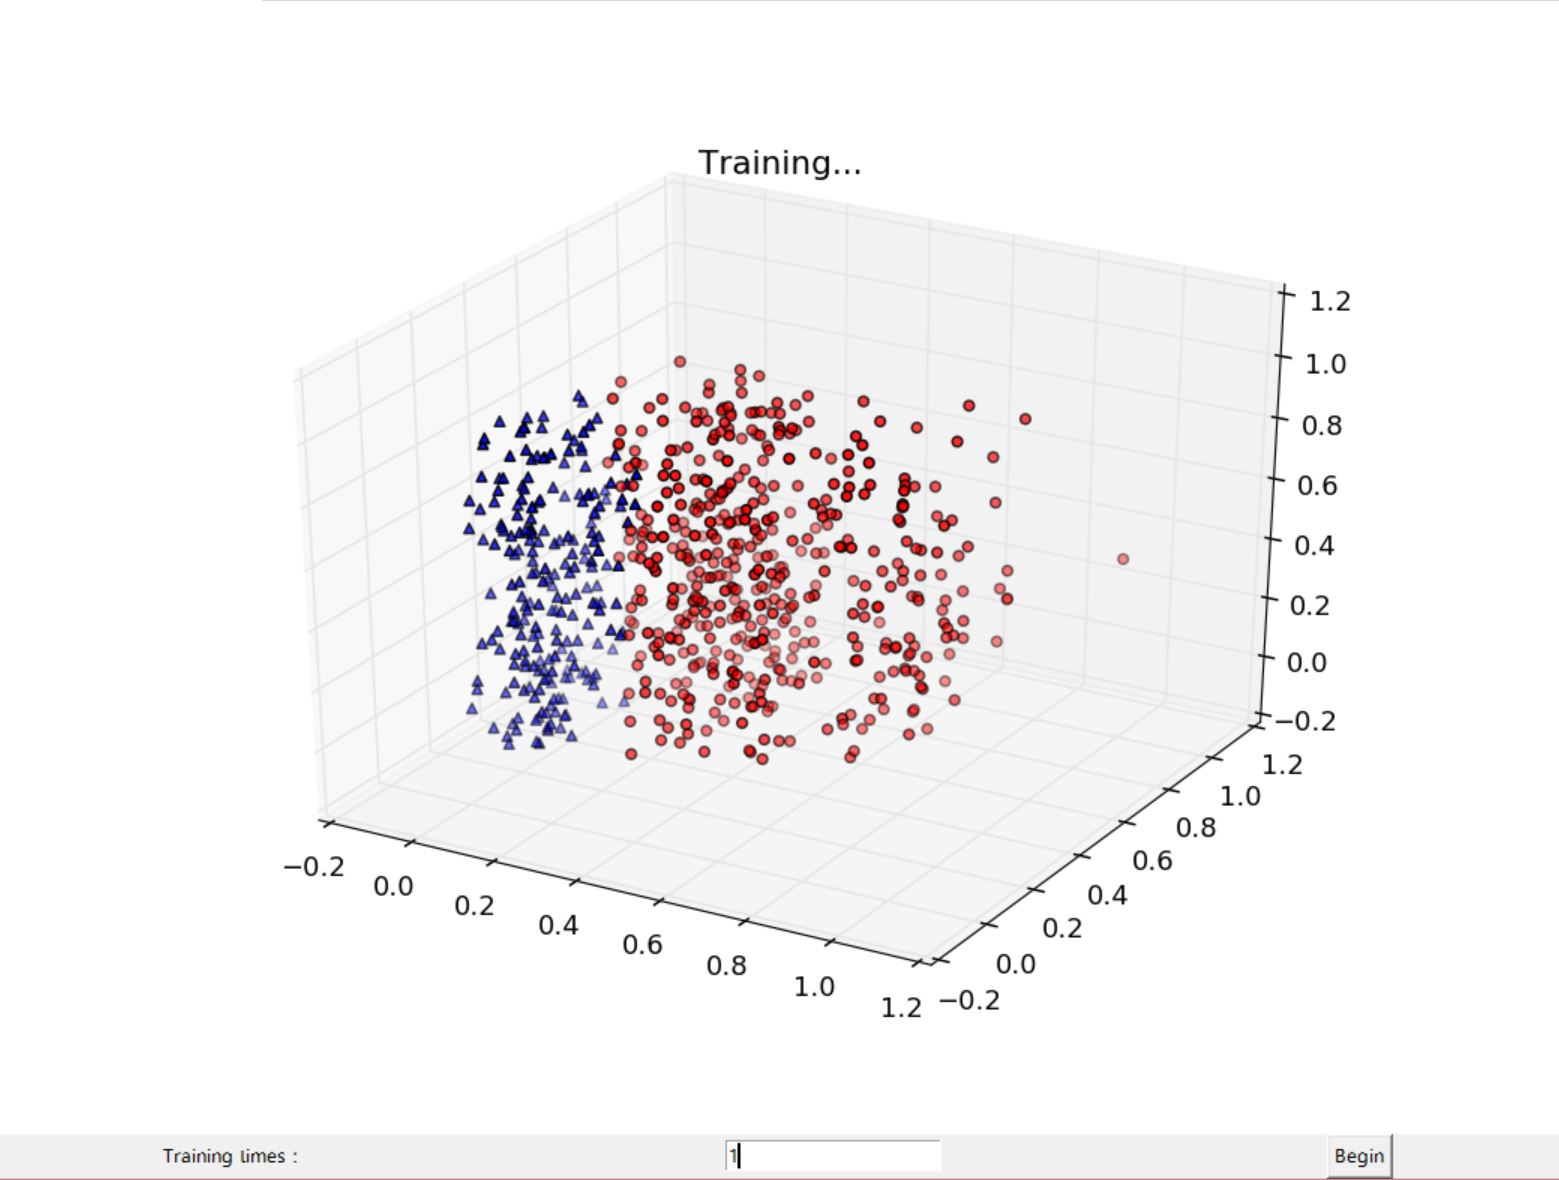
\includegraphics[width=3.5in]{07.jpg}
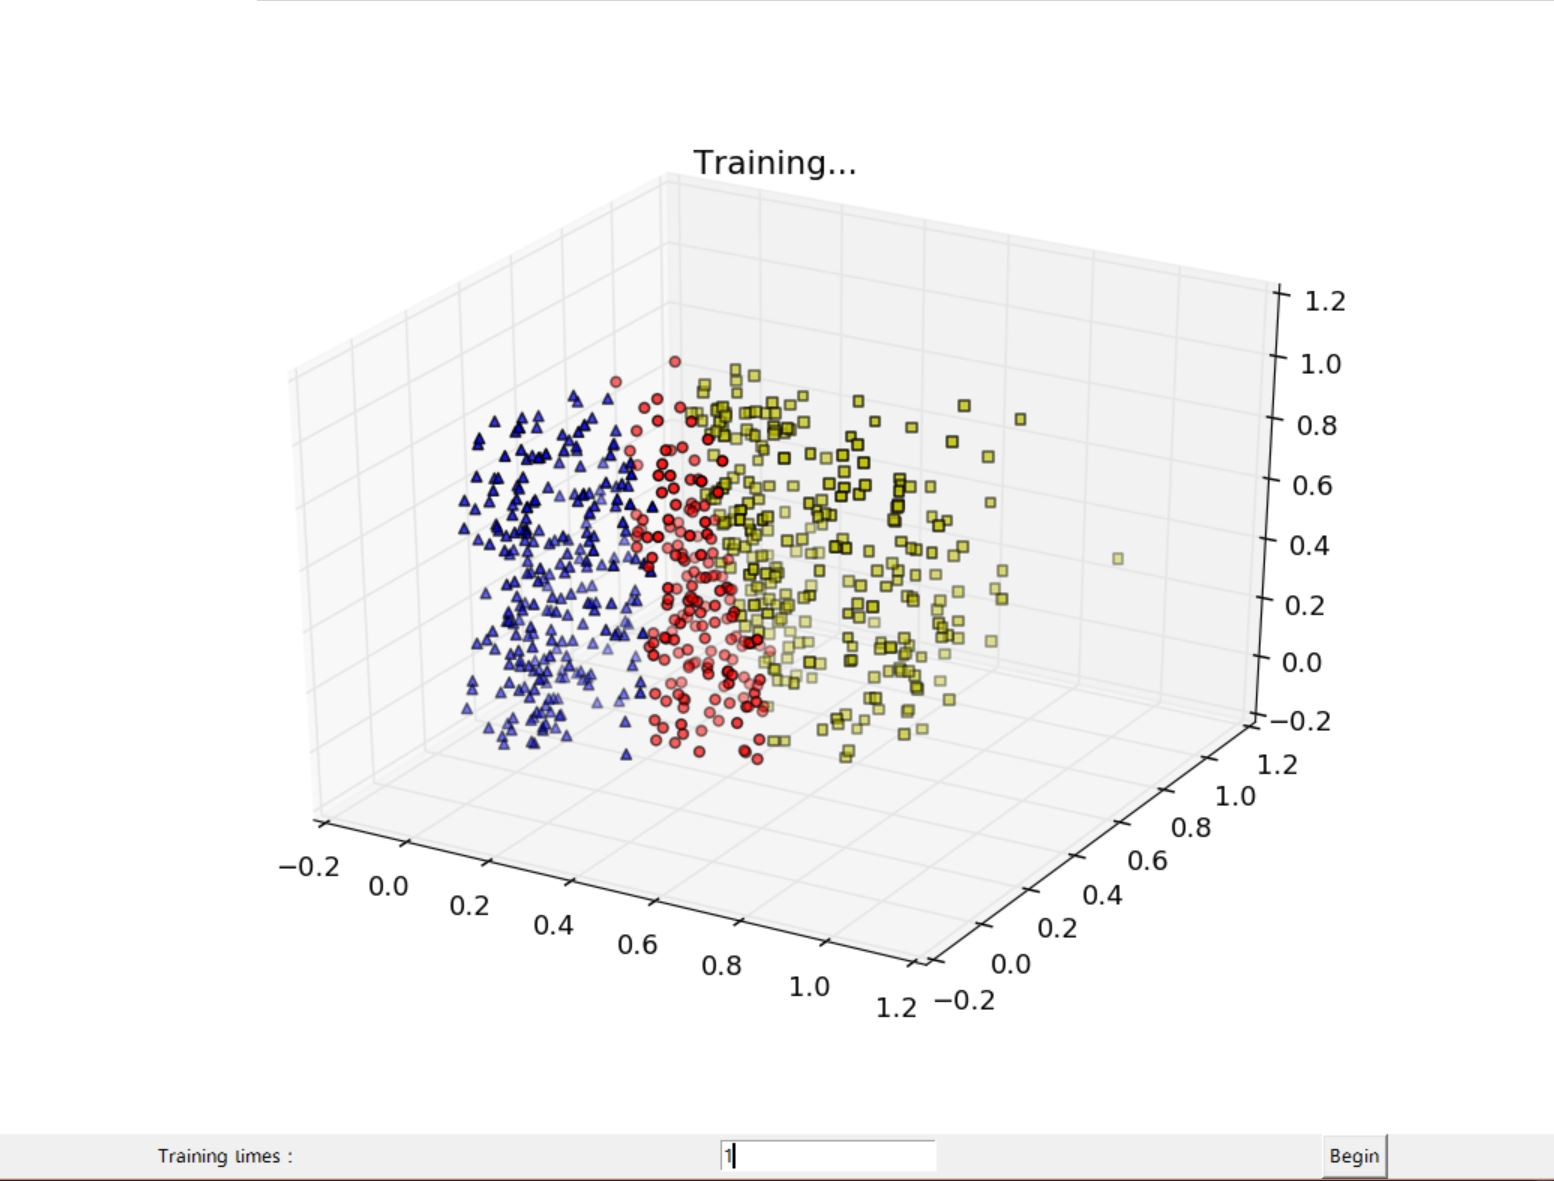
\includegraphics[width=3.5in]{08.jpg}

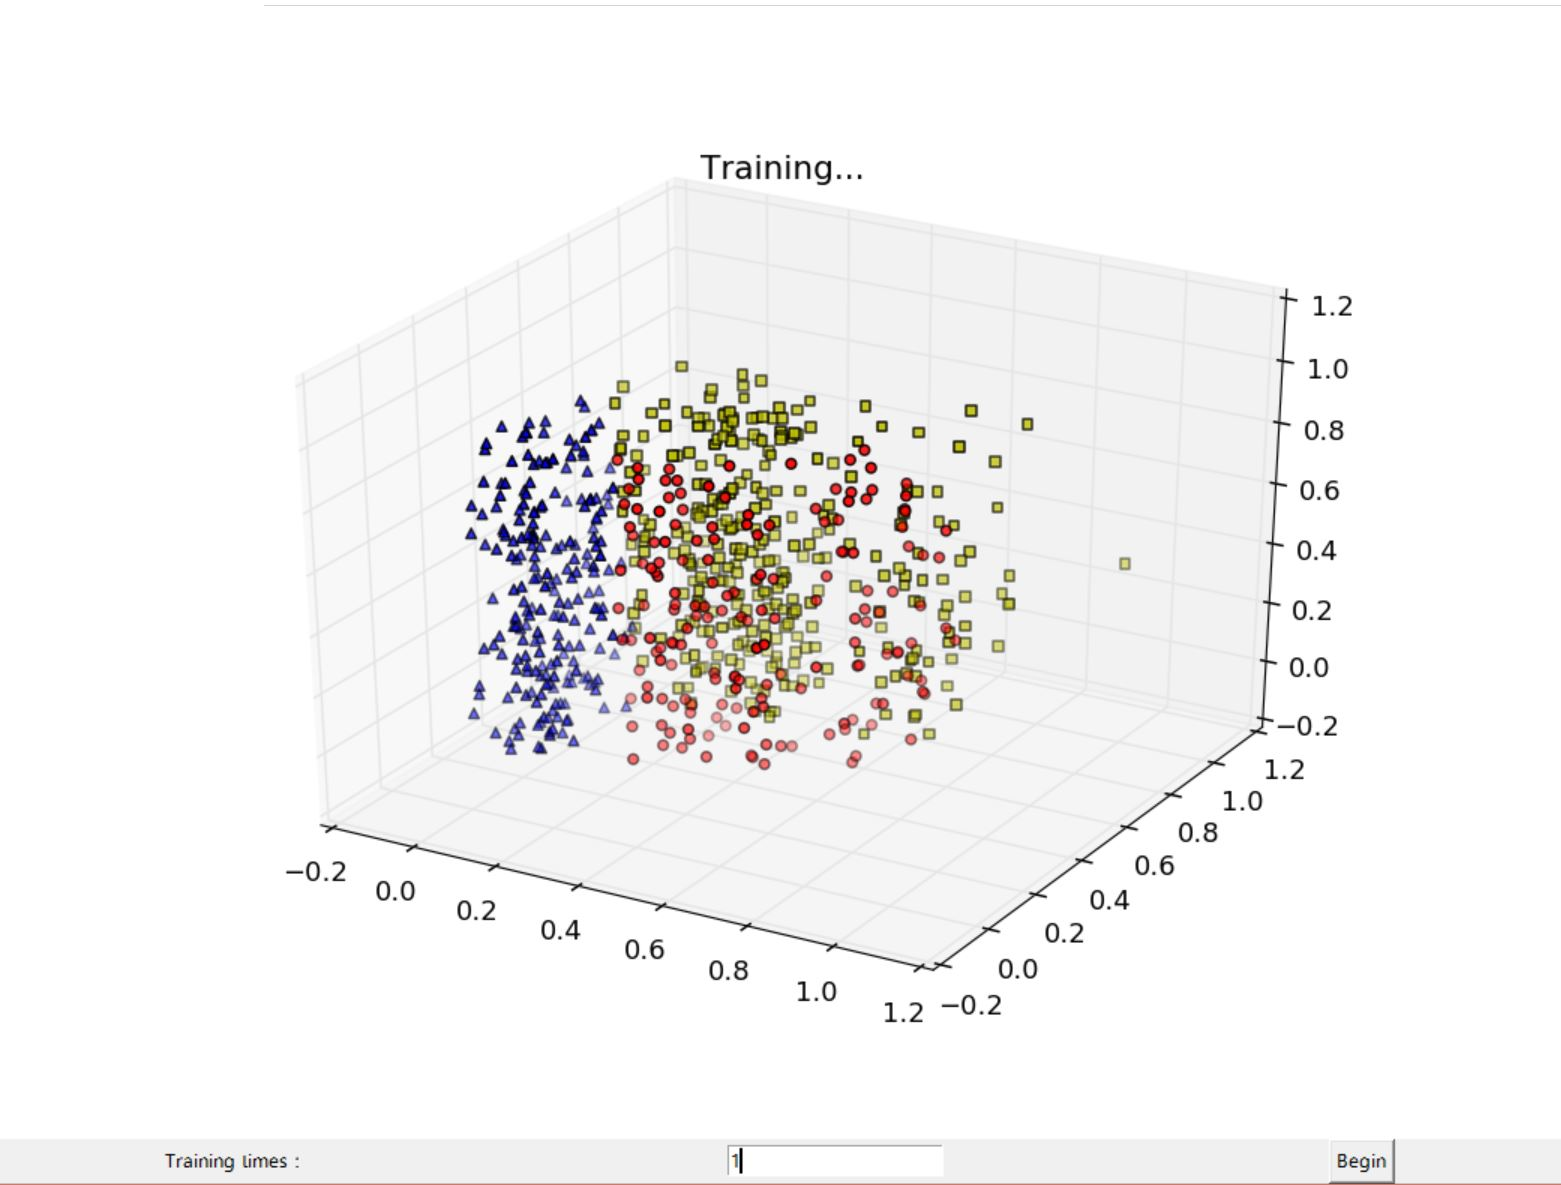
\includegraphics[width=3.5in]{09.jpg}
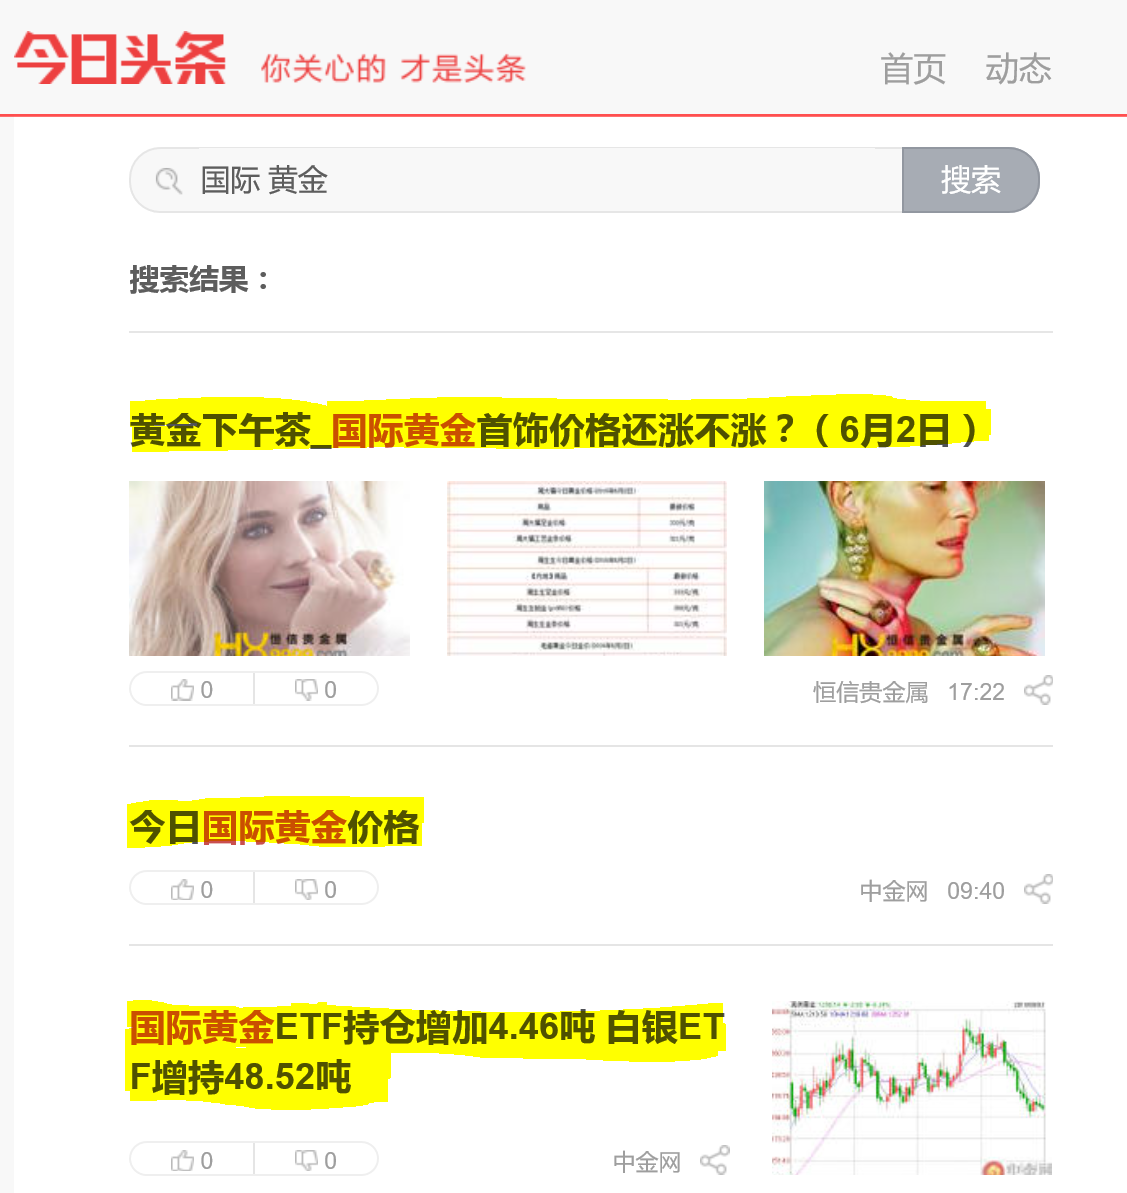
\includegraphics[width=3.5in]{10.jpg}

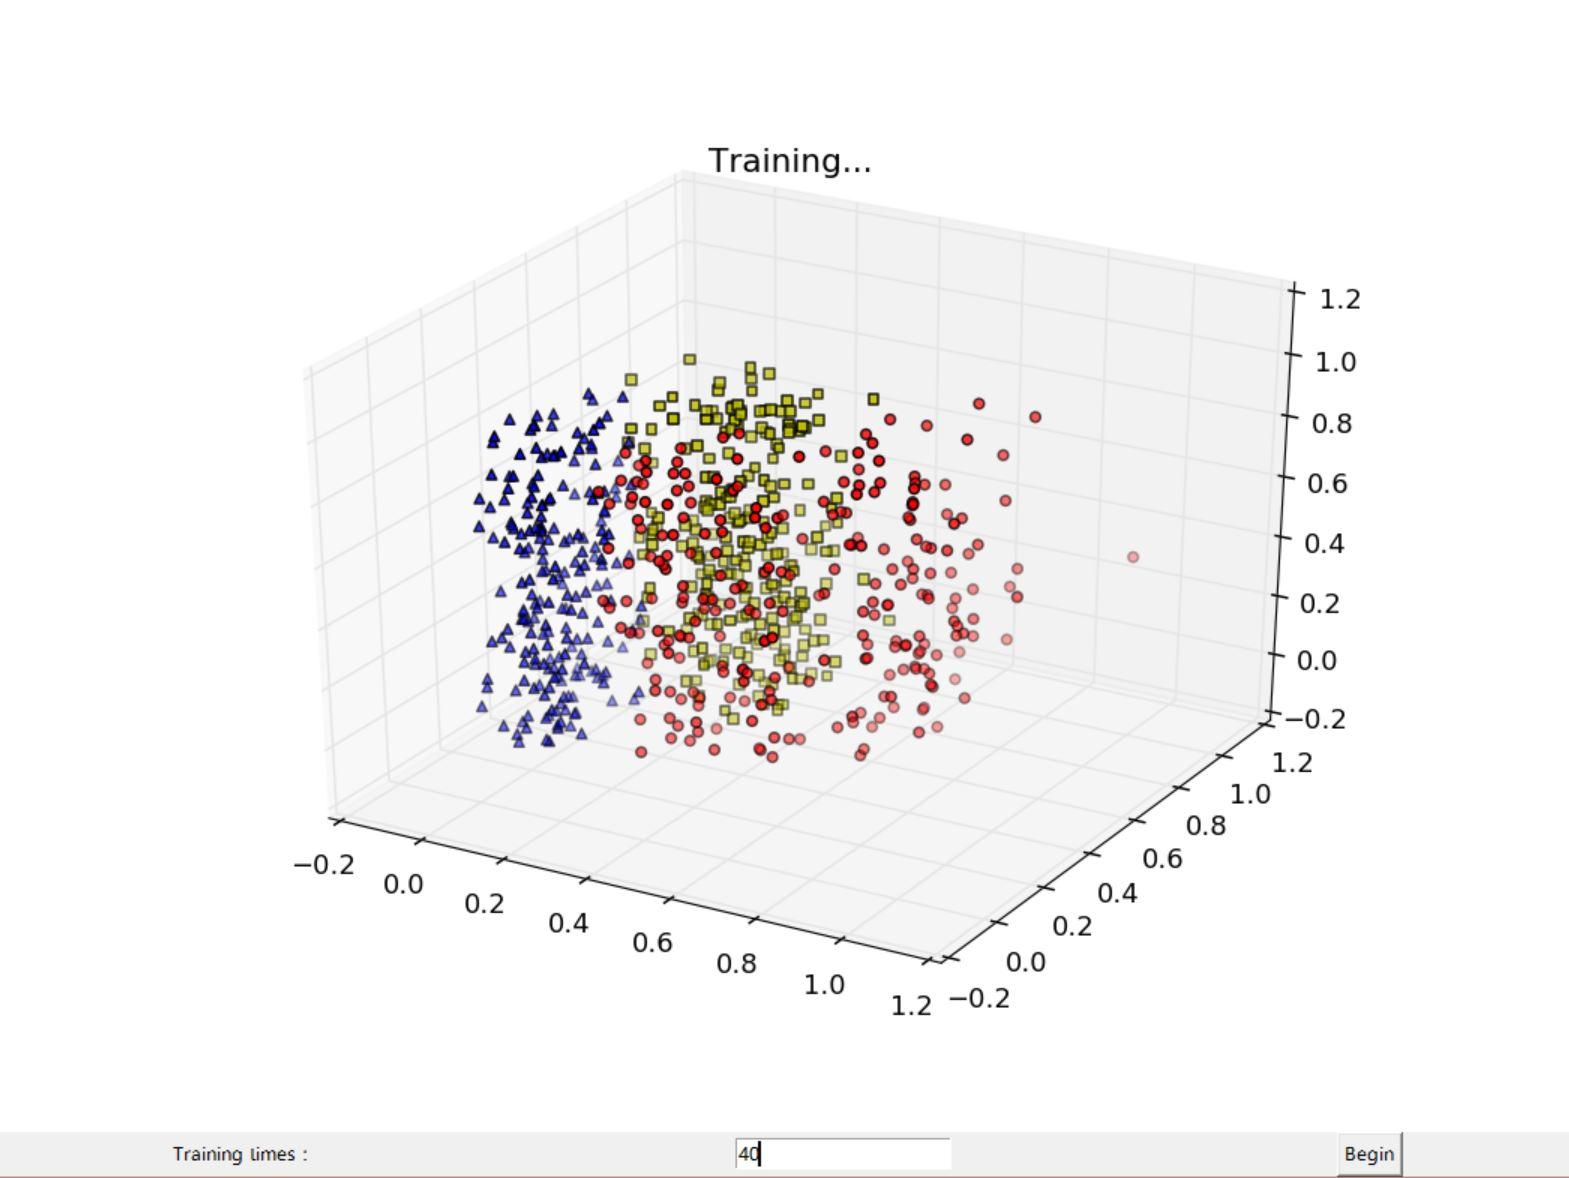
\includegraphics[width=3.5in]{11.jpg}
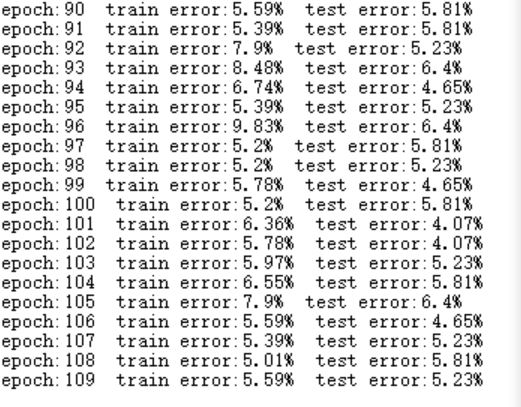
\includegraphics[width=3.5in]{12.jpg}

It works really good. The dataset is the same with kNN method, and now we can see the procession of classifying directly.




%%****************************************
%%  参考文献
%%****************************************
\bibliography{myreference}
\bibliographystyle{plain}
\end{document}  
